% Generated by Sphinx.
\def\sphinxdocclass{report}
\documentclass[letterpaper,10pt,english]{sphinxmanual}
\usepackage[utf8]{inputenc}
\DeclareUnicodeCharacter{00A0}{\nobreakspace}
\usepackage{cmap}
\usepackage[T1]{fontenc}
\usepackage{amsfonts}
\usepackage{babel}
\usepackage{times}
\usepackage[Bjarne]{fncychap}
\usepackage{longtable}
\usepackage{sphinx}
\usepackage{multirow}
\usepackage{eqparbox}


\addto\captionsenglish{\renewcommand{\figurename}{Fig. }}
\addto\captionsenglish{\renewcommand{\tablename}{Table }}
\SetupFloatingEnvironment{literal-block}{name=Listing }



\title{Comenzando con GitHub Documentación}
\date{September 12, 2016}
\release{1.0}
\author{Igor F. Dávalos Rojas}
\newcommand{\sphinxlogo}{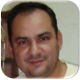
\includegraphics{igor.jpg}\par}
\renewcommand{\releasename}{Release}
\setcounter{tocdepth}{1}
\makeindex

\makeatletter
\def\PYG@reset{\let\PYG@it=\relax \let\PYG@bf=\relax%
    \let\PYG@ul=\relax \let\PYG@tc=\relax%
    \let\PYG@bc=\relax \let\PYG@ff=\relax}
\def\PYG@tok#1{\csname PYG@tok@#1\endcsname}
\def\PYG@toks#1+{\ifx\relax#1\empty\else%
    \PYG@tok{#1}\expandafter\PYG@toks\fi}
\def\PYG@do#1{\PYG@bc{\PYG@tc{\PYG@ul{%
    \PYG@it{\PYG@bf{\PYG@ff{#1}}}}}}}
\def\PYG#1#2{\PYG@reset\PYG@toks#1+\relax+\PYG@do{#2}}

\expandafter\def\csname PYG@tok@gd\endcsname{\def\PYG@tc##1{\textcolor[rgb]{0.63,0.00,0.00}{##1}}}
\expandafter\def\csname PYG@tok@gu\endcsname{\let\PYG@bf=\textbf\def\PYG@tc##1{\textcolor[rgb]{0.50,0.00,0.50}{##1}}}
\expandafter\def\csname PYG@tok@gt\endcsname{\def\PYG@tc##1{\textcolor[rgb]{0.00,0.27,0.87}{##1}}}
\expandafter\def\csname PYG@tok@gs\endcsname{\let\PYG@bf=\textbf}
\expandafter\def\csname PYG@tok@gr\endcsname{\def\PYG@tc##1{\textcolor[rgb]{1.00,0.00,0.00}{##1}}}
\expandafter\def\csname PYG@tok@cm\endcsname{\let\PYG@it=\textit\def\PYG@tc##1{\textcolor[rgb]{0.25,0.50,0.56}{##1}}}
\expandafter\def\csname PYG@tok@vg\endcsname{\def\PYG@tc##1{\textcolor[rgb]{0.73,0.38,0.84}{##1}}}
\expandafter\def\csname PYG@tok@vi\endcsname{\def\PYG@tc##1{\textcolor[rgb]{0.73,0.38,0.84}{##1}}}
\expandafter\def\csname PYG@tok@mh\endcsname{\def\PYG@tc##1{\textcolor[rgb]{0.13,0.50,0.31}{##1}}}
\expandafter\def\csname PYG@tok@cs\endcsname{\def\PYG@tc##1{\textcolor[rgb]{0.25,0.50,0.56}{##1}}\def\PYG@bc##1{\setlength{\fboxsep}{0pt}\colorbox[rgb]{1.00,0.94,0.94}{\strut ##1}}}
\expandafter\def\csname PYG@tok@ge\endcsname{\let\PYG@it=\textit}
\expandafter\def\csname PYG@tok@vc\endcsname{\def\PYG@tc##1{\textcolor[rgb]{0.73,0.38,0.84}{##1}}}
\expandafter\def\csname PYG@tok@il\endcsname{\def\PYG@tc##1{\textcolor[rgb]{0.13,0.50,0.31}{##1}}}
\expandafter\def\csname PYG@tok@go\endcsname{\def\PYG@tc##1{\textcolor[rgb]{0.20,0.20,0.20}{##1}}}
\expandafter\def\csname PYG@tok@cp\endcsname{\def\PYG@tc##1{\textcolor[rgb]{0.00,0.44,0.13}{##1}}}
\expandafter\def\csname PYG@tok@gi\endcsname{\def\PYG@tc##1{\textcolor[rgb]{0.00,0.63,0.00}{##1}}}
\expandafter\def\csname PYG@tok@gh\endcsname{\let\PYG@bf=\textbf\def\PYG@tc##1{\textcolor[rgb]{0.00,0.00,0.50}{##1}}}
\expandafter\def\csname PYG@tok@ni\endcsname{\let\PYG@bf=\textbf\def\PYG@tc##1{\textcolor[rgb]{0.84,0.33,0.22}{##1}}}
\expandafter\def\csname PYG@tok@nl\endcsname{\let\PYG@bf=\textbf\def\PYG@tc##1{\textcolor[rgb]{0.00,0.13,0.44}{##1}}}
\expandafter\def\csname PYG@tok@nn\endcsname{\let\PYG@bf=\textbf\def\PYG@tc##1{\textcolor[rgb]{0.05,0.52,0.71}{##1}}}
\expandafter\def\csname PYG@tok@no\endcsname{\def\PYG@tc##1{\textcolor[rgb]{0.38,0.68,0.84}{##1}}}
\expandafter\def\csname PYG@tok@na\endcsname{\def\PYG@tc##1{\textcolor[rgb]{0.25,0.44,0.63}{##1}}}
\expandafter\def\csname PYG@tok@nb\endcsname{\def\PYG@tc##1{\textcolor[rgb]{0.00,0.44,0.13}{##1}}}
\expandafter\def\csname PYG@tok@nc\endcsname{\let\PYG@bf=\textbf\def\PYG@tc##1{\textcolor[rgb]{0.05,0.52,0.71}{##1}}}
\expandafter\def\csname PYG@tok@nd\endcsname{\let\PYG@bf=\textbf\def\PYG@tc##1{\textcolor[rgb]{0.33,0.33,0.33}{##1}}}
\expandafter\def\csname PYG@tok@ne\endcsname{\def\PYG@tc##1{\textcolor[rgb]{0.00,0.44,0.13}{##1}}}
\expandafter\def\csname PYG@tok@nf\endcsname{\def\PYG@tc##1{\textcolor[rgb]{0.02,0.16,0.49}{##1}}}
\expandafter\def\csname PYG@tok@si\endcsname{\let\PYG@it=\textit\def\PYG@tc##1{\textcolor[rgb]{0.44,0.63,0.82}{##1}}}
\expandafter\def\csname PYG@tok@s2\endcsname{\def\PYG@tc##1{\textcolor[rgb]{0.25,0.44,0.63}{##1}}}
\expandafter\def\csname PYG@tok@nt\endcsname{\let\PYG@bf=\textbf\def\PYG@tc##1{\textcolor[rgb]{0.02,0.16,0.45}{##1}}}
\expandafter\def\csname PYG@tok@nv\endcsname{\def\PYG@tc##1{\textcolor[rgb]{0.73,0.38,0.84}{##1}}}
\expandafter\def\csname PYG@tok@s1\endcsname{\def\PYG@tc##1{\textcolor[rgb]{0.25,0.44,0.63}{##1}}}
\expandafter\def\csname PYG@tok@ch\endcsname{\let\PYG@it=\textit\def\PYG@tc##1{\textcolor[rgb]{0.25,0.50,0.56}{##1}}}
\expandafter\def\csname PYG@tok@m\endcsname{\def\PYG@tc##1{\textcolor[rgb]{0.13,0.50,0.31}{##1}}}
\expandafter\def\csname PYG@tok@gp\endcsname{\let\PYG@bf=\textbf\def\PYG@tc##1{\textcolor[rgb]{0.78,0.36,0.04}{##1}}}
\expandafter\def\csname PYG@tok@sh\endcsname{\def\PYG@tc##1{\textcolor[rgb]{0.25,0.44,0.63}{##1}}}
\expandafter\def\csname PYG@tok@ow\endcsname{\let\PYG@bf=\textbf\def\PYG@tc##1{\textcolor[rgb]{0.00,0.44,0.13}{##1}}}
\expandafter\def\csname PYG@tok@sx\endcsname{\def\PYG@tc##1{\textcolor[rgb]{0.78,0.36,0.04}{##1}}}
\expandafter\def\csname PYG@tok@bp\endcsname{\def\PYG@tc##1{\textcolor[rgb]{0.00,0.44,0.13}{##1}}}
\expandafter\def\csname PYG@tok@c1\endcsname{\let\PYG@it=\textit\def\PYG@tc##1{\textcolor[rgb]{0.25,0.50,0.56}{##1}}}
\expandafter\def\csname PYG@tok@o\endcsname{\def\PYG@tc##1{\textcolor[rgb]{0.40,0.40,0.40}{##1}}}
\expandafter\def\csname PYG@tok@kc\endcsname{\let\PYG@bf=\textbf\def\PYG@tc##1{\textcolor[rgb]{0.00,0.44,0.13}{##1}}}
\expandafter\def\csname PYG@tok@c\endcsname{\let\PYG@it=\textit\def\PYG@tc##1{\textcolor[rgb]{0.25,0.50,0.56}{##1}}}
\expandafter\def\csname PYG@tok@mf\endcsname{\def\PYG@tc##1{\textcolor[rgb]{0.13,0.50,0.31}{##1}}}
\expandafter\def\csname PYG@tok@err\endcsname{\def\PYG@bc##1{\setlength{\fboxsep}{0pt}\fcolorbox[rgb]{1.00,0.00,0.00}{1,1,1}{\strut ##1}}}
\expandafter\def\csname PYG@tok@mb\endcsname{\def\PYG@tc##1{\textcolor[rgb]{0.13,0.50,0.31}{##1}}}
\expandafter\def\csname PYG@tok@ss\endcsname{\def\PYG@tc##1{\textcolor[rgb]{0.32,0.47,0.09}{##1}}}
\expandafter\def\csname PYG@tok@sr\endcsname{\def\PYG@tc##1{\textcolor[rgb]{0.14,0.33,0.53}{##1}}}
\expandafter\def\csname PYG@tok@mo\endcsname{\def\PYG@tc##1{\textcolor[rgb]{0.13,0.50,0.31}{##1}}}
\expandafter\def\csname PYG@tok@kd\endcsname{\let\PYG@bf=\textbf\def\PYG@tc##1{\textcolor[rgb]{0.00,0.44,0.13}{##1}}}
\expandafter\def\csname PYG@tok@mi\endcsname{\def\PYG@tc##1{\textcolor[rgb]{0.13,0.50,0.31}{##1}}}
\expandafter\def\csname PYG@tok@kn\endcsname{\let\PYG@bf=\textbf\def\PYG@tc##1{\textcolor[rgb]{0.00,0.44,0.13}{##1}}}
\expandafter\def\csname PYG@tok@cpf\endcsname{\let\PYG@it=\textit\def\PYG@tc##1{\textcolor[rgb]{0.25,0.50,0.56}{##1}}}
\expandafter\def\csname PYG@tok@kr\endcsname{\let\PYG@bf=\textbf\def\PYG@tc##1{\textcolor[rgb]{0.00,0.44,0.13}{##1}}}
\expandafter\def\csname PYG@tok@s\endcsname{\def\PYG@tc##1{\textcolor[rgb]{0.25,0.44,0.63}{##1}}}
\expandafter\def\csname PYG@tok@kp\endcsname{\def\PYG@tc##1{\textcolor[rgb]{0.00,0.44,0.13}{##1}}}
\expandafter\def\csname PYG@tok@w\endcsname{\def\PYG@tc##1{\textcolor[rgb]{0.73,0.73,0.73}{##1}}}
\expandafter\def\csname PYG@tok@kt\endcsname{\def\PYG@tc##1{\textcolor[rgb]{0.56,0.13,0.00}{##1}}}
\expandafter\def\csname PYG@tok@sc\endcsname{\def\PYG@tc##1{\textcolor[rgb]{0.25,0.44,0.63}{##1}}}
\expandafter\def\csname PYG@tok@sb\endcsname{\def\PYG@tc##1{\textcolor[rgb]{0.25,0.44,0.63}{##1}}}
\expandafter\def\csname PYG@tok@k\endcsname{\let\PYG@bf=\textbf\def\PYG@tc##1{\textcolor[rgb]{0.00,0.44,0.13}{##1}}}
\expandafter\def\csname PYG@tok@se\endcsname{\let\PYG@bf=\textbf\def\PYG@tc##1{\textcolor[rgb]{0.25,0.44,0.63}{##1}}}
\expandafter\def\csname PYG@tok@sd\endcsname{\let\PYG@it=\textit\def\PYG@tc##1{\textcolor[rgb]{0.25,0.44,0.63}{##1}}}

\def\PYGZbs{\char`\\}
\def\PYGZus{\char`\_}
\def\PYGZob{\char`\{}
\def\PYGZcb{\char`\}}
\def\PYGZca{\char`\^}
\def\PYGZam{\char`\&}
\def\PYGZlt{\char`\<}
\def\PYGZgt{\char`\>}
\def\PYGZsh{\char`\#}
\def\PYGZpc{\char`\%}
\def\PYGZdl{\char`\$}
\def\PYGZhy{\char`\-}
\def\PYGZsq{\char`\'}
\def\PYGZdq{\char`\"}
\def\PYGZti{\char`\~}
% for compatibility with earlier versions
\def\PYGZat{@}
\def\PYGZlb{[}
\def\PYGZrb{]}
\makeatother

\renewcommand\PYGZsq{\textquotesingle}

\begin{document}

\maketitle
\tableofcontents
\phantomsection\label{index::doc}



\part{PARTE: INTRODUCCIÓN}
\label{introduccion:introduccion}\label{introduccion:parte-introduccion}\label{introduccion:welcome-to-comenzando-con-github-s-documentation}\label{introduccion::doc}

\chapter{CAPÍTULO: BREVES COMENTARIOS SOBRE ESTA COSA}
\label{introduccion:capitulo-breves-comentarios-sobre-esta-cosa}\label{introduccion:capitulo1}
Todo tiene un comienzo, no siempre agradable, en una idea que se forma en la cabezota de alguien
en este caso se formó en la \emph{cabezota mía} como parte de mi curiosidad innata de \emph{saber cómo} funcionan las cosas.
Hablando claro, en este caso, de la forma en que fue elaborado el Manual del Usuario de SCP.


\chapter{CAPÍTULO: AQUÍ PONDRÉ OTRO CAPÍTULO}
\label{introduccion:capitulo2}\label{introduccion:capitulo-aqui-pondre-otro-capitulo}
A no ser que se ponga como capítulo. Esto de estar aprendiendo es divertido para mí y una distracción en estos momentos de ociosidad.


\part{PARTE: ¿SEGUNDA PARTE?}
\label{introduccion:parte-segunda-parte}\label{introduccion:segundaparte}

\chapter{CAPÍTULO: SEGUNDO DE LA SEGUNDA PARTE}
\label{introduccion:capitulo-segundo-de-la-segunda-parte}\label{introduccion:capitulo1-2}
¿Será que así que se van estructurando las partes y los capítulos?

Una imagen suelta

\includegraphics[width=100pt]{{igor2}.jpg}


\section{Si coloco otro caracter ¿cómo se estructura?}
\label{introduccion:si-coloco-otro-caracter-como-se-estructura}\label{introduccion:colocarnum}
No aparece nada.

Con los cambios que hice, ya apareció. Falta la numeración.


\section{Con estos cambios debería aparecer la numeración}
\label{introduccion:cambiosrec}\label{introduccion:con-estos-cambios-deberia-aparecer-la-numeracion}
Realicé nuevos cambios. Voy a insertar una ecuación, luego buscaré sobre sintaxis de las ecuaciones mathjax.

Una ecuación en su propia línea:
\begin{gather}
\begin{split}X = A_b + Z^2\end{split}\notag
\end{gather}
Una ecuación en línea con el texto sería \(H^2 = L_a * L_b\) y después seguiría escribiento texto.

No consigo que se muestre la numeración de las secciones


\section{Primeras referencias}
\label{introduccion:primeras-referencias}
Ir a {\hyperref[introduccion:introduccion]{\emph{PARTE: INTRODUCCIÓN}}} (\autopageref*{introduccion:introduccion}) para mayores detalles

O directamente al {\hyperref[introduccion:capitulo1]{\emph{CAPÍTULO: BREVES COMENTARIOS SOBRE ESTA COSA}}} (\autopageref*{introduccion:capitulo1}) que es donde comienza todo.


\part{Referencias}
\label{imagenes:referencias}\label{imagenes::doc}
¿Se volvió Capítulo?


\chapter{CAPÍTULO: USANDO MÁS COSAS}
\label{imagenes:capitulo-usando-mas-cosas}

\section{Listas sin orden}
\label{imagenes:listas-sin-orden}
Primer listado:
\begin{itemize}
\item {} 
Elemento 1

\item {} 
Elemento 2

\item {} 
Elemento 3
\begin{itemize}
\item {} 
Elemento 1

\item {} 
Elemento 2

\item {} 
Elemento 3

\end{itemize}

\item {} 
Elemento 4

\item {} 
Elemento 5

\end{itemize}

Se acabó la lista desordenada. Ir al {\hyperref[introduccion:capitulo2]{\emph{CAPÍTULO: AQUÍ PONDRÉ OTRO CAPÍTULO}}} (\autopageref*{introduccion:capitulo2}).


\section{Listas ordenadas}
\label{imagenes:listas-ordenadas}\begin{enumerate}
\item {} 
Artículo 1

\item {} 
Artículo 2

\item {} 
Artículo 3
\begin{enumerate}
\item {} 
Sub Artículo 1

\item {} 
Sub Artículo 2

\end{enumerate}

\item {} 
Artículo 4

\end{enumerate}

\textbf{Ahora a usar Sphinx para ver el pdf.}
\begin{description}
\item[{RST}] \leavevmode
Lenguaje de marcado de texto para elaborar documentos desde sencillos hasta complejos utilizando el marcado de texto.

\item[{SPHINX}] \leavevmode
Permite construir un documento basado en RST.

\end{description}

Se acabó la definición.

\begin{DUlineblock}{0em}
\item[] ¿Líneas como
\item[] en el código?
\item[] veremos
\end{DUlineblock}

Ahora a ensayar bloques literales que permiten mostrar en el documento construido el texto tal y como aparece en el código

\begin{Verbatim}[commandchars=\\\{\}]
Esta es la primer línea de código
Seguda línea
Tercer y última línea

Dos líneas en un
nuevo párrafo
\end{Verbatim}

Ahora texto supuestamente normal. Voy a escribir lo que salga con tal de que ocupe por lo menos dos líneas en el documento
ensamblado (será ese el nombre correcto?).


\part{PROVINCIAS DEL BENI}
\label{provincias::doc}\label{provincias:provincias-del-beni}\label{provincias:provincias}

\chapter{Provincia Cercado}
\label{cercado::doc}\label{cercado:provincia-cercado}\label{cercado:cercado}
Está dividida en dos Municipio, \emph{Municipio de Trinidad} y \emph{Municipio de San Javier}.
Capital Trinidad, que tambiéne s Capital del Departamento del Beni y del Municipio de Trinidad.


\section{Municipio de Trinidad}
\label{cercado:municipio-de-trinidad}\label{cercado:mun-trinidad}
Se dice mucho de estooo  y bla bla bla bla bla bla.


\subsection{Ciudad de la Santísima Trinidad}
\label{cercado:ciudad-de-la-santisima-trinidad}\label{cercado:trinidad}
Ubicada en la {\hyperref[cercado:cercado]{\emph{Provincia Cercado}}} (\autopageref*{cercado:cercado}) Capital del Departamento del Beni.

Bla bla bla bla bla bla bla bla bla bla bla bla bla bla bla bla bla bla bla bla bla bla bla bla bla bla bla bla bla bla bla bla bla bla
bla bla bla bla bla bla bla bla bla bla bla bla bla bla bla bla bla bla bla bla bla bla bla bla bla bla bla
bla bla bla bla bla bla bla bla bla bla bla bla bla bla bla bla bla bla bla bla bla bla bla bla bla bla bla op
bla bla bla bla bla bla bla bla bla bla bla bla bla bla bla bla bla bla bla bla bla bla bla bla bla bla bla 8uyyyy
bla bla bla bla bla bla bla bla bla bla bla bla bla bla bla bla bla bla bla bla bla bla bla bla bla bla bla.


\subsection{Localidad de San Javier}
\label{cercado:san-javier}\label{cercado:localidad-de-san-javier}
Ubicada en la {\hyperref[cercado:cercado]{\emph{Provincia Cercado}}} (\autopageref*{cercado:cercado}) Capital del Departamento del Beni.

Bla bla bla bla bla bla bla bla bla bla bla bla bla bla bla bla bla bla bla bla bla bla bla bla bla bla bla bla bla bla bla bla bla bla
bla bla bla bla bla bla bla bla bla bla bla bla bla bla bla bla bla bla bla bla bla bla bla bla bla bla bla
bla bla bla bla bla bla bla bla bla bla bla bla bla bla bla bla bla bla bla bla bla bla bla bla bla bla bla op
bla bla bla bla bla bla bla bla bla bla bla bla bla bla bla bla bla bla bla bla bla bla bla bla bla bla bla 8uyyyy
bla bla bla bla bla bla bla bla bla bla bla bla bla bla bla bla bla bla bla bla bla bla bla bla bla bla bla.


\chapter{Provincia Marbán}
\label{marban:provincia-marban}\label{marban::doc}\label{marban:marban}
Divida en dos Municipios, \emph{Loreto{}`y {}`San Andrés}.


\section{Municipio de Loreto}
\label{marban:municipio-de-loreto}\label{marban:mun-loreto}
Se dice mucho de estooo  y bla bla bla bla bla bla.


\subsection{Ciudad de Loreto}
\label{marban:loreto}\label{marban:ciudad-de-loreto}
Ubicada en la {\hyperref[marban:marban]{\emph{Provincia Marbán}}} (\autopageref*{marban:marban}) Capital del Departamento del Beni.

Bla bla bla bla bla bla bla bla bla bla bla bla bla bla bla bla bla bla bla bla bla bla bla bla bla bla bla bla bla bla bla bla bla bla
bla bla bla bla bla bla bla bla bla bla bla bla bla bla bla bla bla bla bla bla bla bla bla bla bla bla bla
bla bla bla bla bla bla bla bla bla bla bla bla bla bla bla bla bla bla bla bla bla bla bla bla bla bla bla op
bla bla bla bla bla bla bla bla bla bla bla bla bla bla bla bla bla bla bla bla bla bla bla bla bla bla bla 8uyyyy
bla bla bla bla bla bla bla bla bla bla bla bla bla bla bla bla bla bla bla bla bla bla bla bla bla bla bla.


\subsection{Localidad de San Andrés}
\label{marban:san-andres}\label{marban:localidad-de-san-andres}
Ubicada en la {\hyperref[marban:marban]{\emph{Provincia Marbán}}} (\autopageref*{marban:marban}) Capital del Departamento del Beni.

Bla bla bla bla bla bla bla bla bla bla bla bla bla bla bla bla bla bla bla bla bla bla bla bla bla bla bla bla bla bla bla bla bla bla
bla bla bla bla bla bla bla bla bla bla bla bla bla bla bla bla bla bla bla bla bla bla bla bla bla bla bla
bla bla bla bla bla bla bla bla bla bla bla bla bla bla bla bla bla bla bla bla bla bla bla bla bla bla bla op
bla bla bla bla bla bla bla bla bla bla bla bla bla bla bla bla bla bla bla bla bla bla bla bla bla bla bla 8uyyyy
bla bla bla bla bla bla bla bla bla bla bla bla bla bla bla bla bla bla bla bla bla bla bla bla bla bla bla.

Forma parte de las {\hyperref[provincias:provincias]{\emph{PROVINCIAS DEL BENI}}} (\autopageref*{provincias:provincias}) que actualmente forman parte de la División Político Administrativa de Bolivia.

\textbf{Todavía no consigo que salgan numerados los títulos}

La fórmula sería: \(Sale - Nosale = NoSabe\) es decir, que no sé cómo hacerlo.

A seguir leyendo.

\emph{¿será que es necesario tocar algún archivo de configuración de Latex?}

\emph{O ¿del documentClass?}

\textbf{Ya me congelé...}

Mier.....

Comenzando el \textbf{sampledoc} de \emph{John Hunter, Fernando Perez, Michael Droettboom}



\renewcommand{\indexname}{Index}
\printindex
\end{document}
